\documentclass[12pt,a4paper,DIV=9]{scrartcl}
\usepackage{pgf}
\usepackage{tikz}
\usetikzlibrary{arrows,automata,positioning}
\usepackage{ngerman}
\usepackage[utf8]{inputenc}
\usepackage{amsmath,amssymb}
\usetikzlibrary{shapes,snakes}
% Schriftart ändern
\renewcommand{\rmdefault}{ppl}
%Möglichkeit zur Änderung von Überschriften
\usepackage{sectsty}
%Überschrift \section uandern
\definecolor{blue}{RGB}{76 , 92, 153}
\allsectionsfont{\color{blue}}
\paragraphfont{\color{blue}}

%Variable Blattnummer
\newcommand{\blatt}[1]{
  \newcommand{\blattnr}{#1}
}
%Aufgabe und Aufgabenteil definieren
\newcounter{temp}
\newcommand{\aufgabe}[1]{
  \setcounter{temp}{\value{subsection}}
  \setcounter{subsection}{#1}
  \addtocounter{subsection}{-1}
  \subsection{Aufgabe}
  \setcounter{subsection}{\value{temp}}
}
\newcommand{\teil}[2][]{
  \subsubsection*{#2) #1}
}
\renewcommand{\author}[1]{\renewcommand{\author}{#1}}
\renewcommand{\title}[1]{\renewcommand{\title}{#1}}
\newcommand{\makehomeworktitle}{
  \begin{minipage}{6.5cm}
    \sf{\author}
  \end{minipage}
  \begin{minipage}{6.5cm}
    \begin{flushright}
      \sf{\title\\\today}
    \end{flushright}
  \end{minipage}
  \\[0.2cm]
  \begin{center}
    \sf{
      \color{blue}{
        \LARGE{Aufgabenblatt \blattnr}
      }
    }
  \end{center}
  \vspace{0.1cm}
}

%%%%%%%%%%%%%%%%%%%%%%%%
%%% Statisch
\author{{[}4131658{]} Jan Germann \\{[}1234567{]} Christian Ratz}
\title{Relationale Datenbanken 1}

%%% Auf jedes Hausaufgabenblatt anpassen
\blatt{2}
%%%%%%%%%%%%%%%%%%%%%%%%
\setcounter{section}{\blattnr}
\begin{document}
\makehomeworktitle

\aufgabe{1}
\teil{a}
  Die ANSI-SPARC Architektur separiert die Benutzeranwendungen und Views von der physikalischen Datenbank. Sie besteht aus den drei Ebenen 
  \begin{enumerate}
    \item \bf{Darstellungsebene} \\
      Diese Schicht ist extern und nicht direkt ein Teil des DBMS
    \item \bf{logische Ebene} \\
      Hat einen Menschen,  alter, ganz Zahl 
    \item \bf{physikalische Ebene}
      Bestimmt wie, wo daten gespeichert werden und was dort gespeichert wird. Zum Beispiel bestimmt es ob die daten auf platte eins oder platte x liegen. Interne representation von daten, z.B. Integer wird in n Bits abgelegt
    \end{enumerate}
\teil{b}

\aufgabe{2}
\teil{a}
  Ein Entitätstyp ist eine »Struktur« welche allen der Entitäten diesen Typs gemein ist. So ist ein Entitätstyp durch seinen Namen und die Menge seiner Attribute beschrieben.
  Eine Entität repräsentiert ein reales Objekt mit einer unabhängigen Existenz. Die einzelne Entität ist immer eine Instanz eines Entitätstyps.
  \paragraph{Bespiel} Ein Stift, ein Auto, der Nachbar mit Namen »Dieter«, u.v.m.
\teil{b}
\teil{c}
\teil{d}
\teil{a}
\aufgabe{3}
  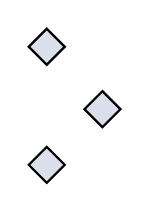
\begin{tikzpicture}[scale=1]

  \tikzset{every node/.style={draw, thick, fill=blue!20}}
    \node (a) [diamond] {};
    \node (b) [diamond] at (45:1cm) {};
    \node (b) [diamond] at (90:1.5cm) {};
  %  \node (b) [diamond, above=3em of a] {};
\end{tikzpicture}

\aufgabe{4}
\aufgabe{5}



\end{document}